\documentclass[CJK]{beamer}
\usepackage{CJKutf8}
\usepackage{graphicx}
\usepackage{tikz}
\usetheme{Copenhagen}
%\usetheme{Boadilla}
\setbeamercovered{transparent}

\usepackage[T1]{fontenc}
\usepackage[default]{gillius}

\begin{document}

\begin{CJK*}{UTF8}{gkai}

\title{Leveldb原理与源码剖析}
\author{youngsterxyf}
\date{2014.08.31}

\begin{frame}[plain]
	\titlepage
\end{frame}

\section{简介}
\begin{frame}{Leveldb简介}
\begin{block}{特点}
	\begin{itemize}
	\item 持久化存储的KV系统
	\item 记录按Key有序存储
	\item 应用场景:写远远多于读
	\item LIB, NO SERVER --- 好处是?
	\item 单进程
	\end{itemize}
\end{block}

\begin{block}{测评}
	\begin{itemize}	
	\item 随机写:40万条记录每秒
	\item 随机读:6万条记录每秒
	\item 顺序读?
	\end{itemize}
\end{block}
\end{frame}

\begin{frame}{应用案例}
\begin{block}{}
	\begin{itemize}
	\item InfluxDB
	\item BigTable
	\item Google Chrome IndexDB
	\item 淘宝Tair的持久化存储引擎
	\item 可作为很多存储方案的存储引擎(如cayley、Riak)
	\item 异步消息队列的Broker
	\end{itemize}
\end{block}
\end{frame}

\section{基本原理}
\begin{frame}{Leveldb基本原理}
\begin{center}
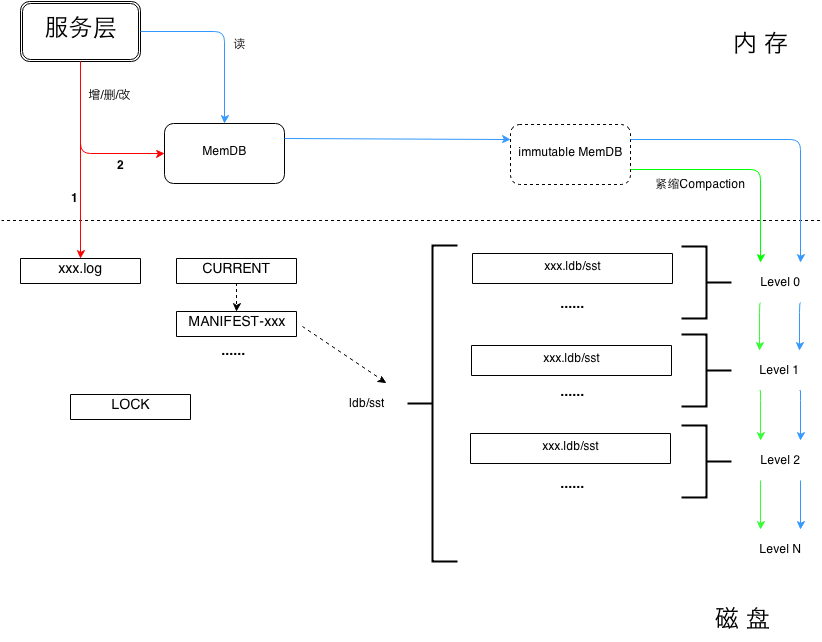
\includegraphics[height=6cm]{leveldb-arch-diagram.png}
\end{center}
\end{frame}

\section{简单实践}
\begin{frame}{LevelDB的使用}
\begin{block}{}
如何使用LevelDB?程序演示... {\color{blue}\href{https://github.com/HappyTechGroup/1st-phase/tree/master/leveldb/code}{源码见Github}}

逐个接口探索实现...
\end{block}
\end{frame}

\section{关键源码剖析}

\subsection{初始化}
\begin{frame}{基本逻辑}

\end{frame}

\subsection{插入}
\begin{frame}{基本逻辑}
\end{frame}

\subsection{紧缩}
\begin{frame}{基本逻辑}
\end{frame}

\subsection{查找}
\begin{frame}{基本逻辑}
\end{frame}

\subsection{删除}
\begin{frame}{基本逻辑}
\end{frame}

\subsection{核心数据结构与算法}
\begin{frame}{跳表skiplist}
\end{frame}

\begin{frame}{布隆过滤器Bloom Filter}
\end{frame}

\begin{frame}{CRC校验}
\end{frame}

\section{参考资料}
\begin{frame}{参考资料}
\begin{itemize}
{\color{blue}
\item \href{http://www.cnblogs.com/haippy/archive/2011/12/04/2276064.html}{数据分析与处理之二(Leveldb 实现原理)}
\item \href{http://leveldb.googlecode.com/svn/trunk/doc/index.html}{Leveldb官方文档}
\item \href{https://code.google.com/p/leveldb/}{Leveldb - Google Code}
\item \href{http://dirlt.com/leveldb.html}{Leveldb - dirlt.com}
}
\end{itemize}
\end{frame}

\begin{frame}{Q \& A}
\begin{center}
谢 谢!
\end{center}
\end{frame}
\end{CJK*}
\end{document}